\section{Zielsetzung}
In diesem Versuch werden Strömungen mittels Doppler-Sonographie untersucht.
Dazu wird mit dem Impuls-Echo-Verfahren die Strömungsgeschwindigkeit sowie das Strömungsprofil bestimmt.

\section{Theoretische Grundlagen}
Bewegen sich eine Schallquelle und ein Schallempfänger relativ zueinander, tritt der Doppler-Effekt, 
eine Änderung der Frequenz auf.

\noindent
Bewegt sich die Quelle auf einen ruhenden Beobachter zu, verschiebt sich die Frequenz $\nu_0$ zu höheren Frequenzen $\nu_{kl}$, 
bzw. verschiebt sich zu tieferen Frequenzen $\nu_{gr}$, wenn sich die Quelle vom Beobachter entfernt.
Somit ist:

\begin{equation}
\nu_{kl/gr} = \frac{\nu_0}{1 \mp \frac{v}{c}}.
\label{eqn:doppler1}
\end{equation}


\noindent
Bewegt sich der Beobachter auf eine ruhende Quelle zu, verschiebt sich die Frequenz $\nu_0$ zu höheren Frequenzen $\nu_h$, 
bzw. verschiebt sich zu tieferen Frequenzen $\nu_{n}$, wenn sich der Beobachter von der Quelle entfernt und es gilt:

\begin{equation}
        \nu_{h/n} = \nu_0 (1 \pm \frac{v}{c}).
        \label{eqn:doppler2}
\end{equation}


\noindent
Der Ultraschall liegt mit Frequenzen von 20 kHz bis ca 1 GHz oberhalb der Hörschwelle und wird in Verbindung mit dem Doppler-Effekt genutzt,
um in der Medizin z.B. die Geschwindigkeit von Blutströmungen zu messen.
Dieses Verfahren ist in Abbildung (\ref{fig:bild}) dargestellt.

\begin{figure}
    \centering
       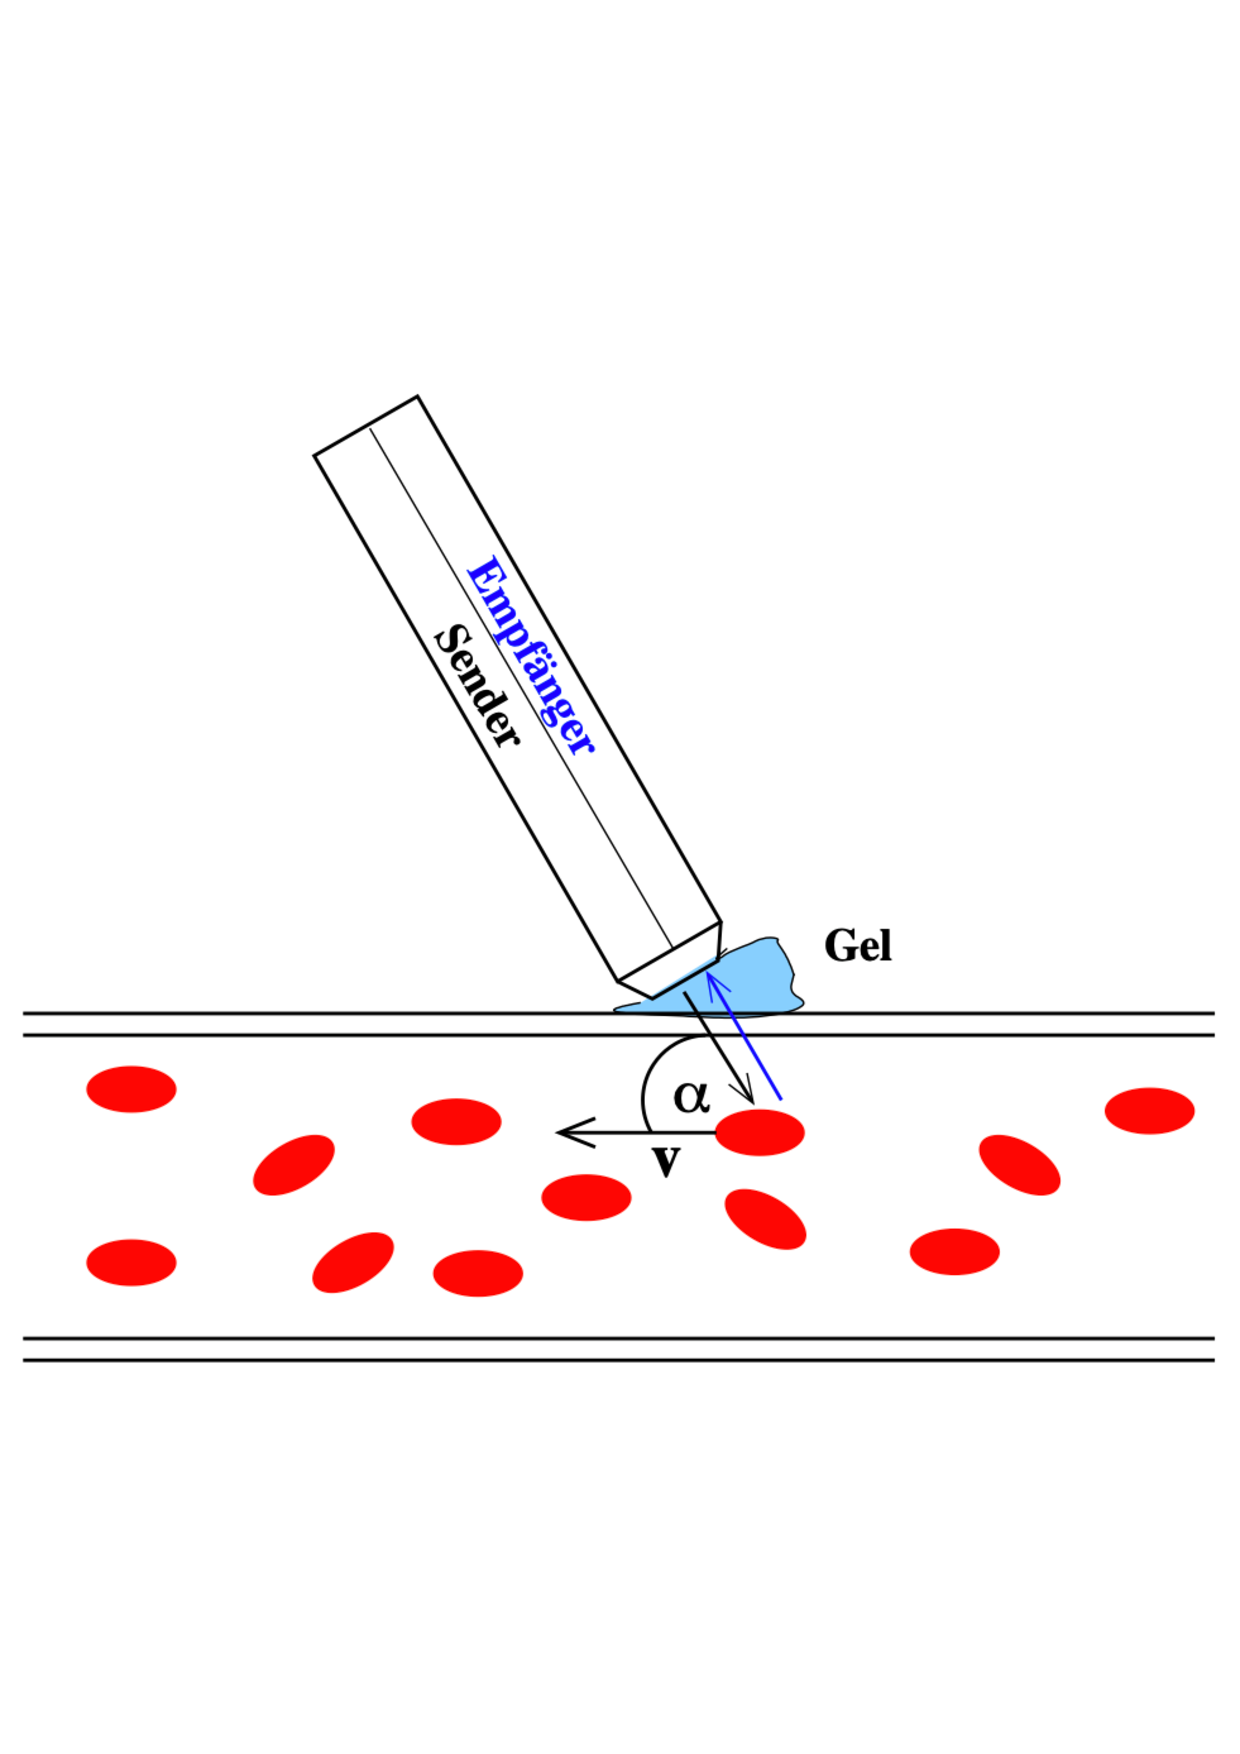
\includegraphics[height=5cm]{bild.pdf}
       \caption{Anwendung des Doppler-Effekts in der Medizin (Quelle: \cite{US3}).}
       \label{fig:bild}
\end{figure}

\noindent
Trifft eine Ultraschallwelle auf einen sich bewegenden Blutkörper, 
verschiebt sich seine Frequenz $\nu$ nach dem Doppler-Effekt um 

\begin{equation}
        \Delta\nu = \nu_0 \frac{v}{c} (cos\,\alpha + cos\,\beta).
\end{equation}

\noindent
Dabei ist v die Geschwindigkeit des sich bewegenden Objekts und c die Schallgeschwindigkeit.
Die Winkel $\alpha$ und $\beta$ liegen zwischen v und der Wellennormalen der einlaufenden/auslaufenden Welle,
die bei dem verwendeten Impuls-Echo Verfahren identisch sind, sodass

\begin{equation}
        \Delta\nu = 2\nu_0 \frac{v}{c} cos\,\alpha
        \label{eqn:dv}
\end{equation}

\noindent
gilt.

\noindent
Die Erzeugung von Ultraschall kann durch die Anwendung des piezo-elektrischen Effekts erfolgen.
Dabei wird ein piezoelektrischer Kristall, häufig Quarz, in einem elektrischen Wechselfeld zum Schwingen angeregt,
sobald eine seiner polaren Achsen in Richtung des elektrischen Felds zeigt.
Beim Schwingen strahlt der Kristall Ultraschallwellen ab, die extrem hohe Schallenergiedichten annehmen können,
wenn die Anregungsfrequenz mit der Eigenfrequenz übereinstimmt und es zur Resonanz kommt.

\noindent
Der Piezokristall kann auch als Schallempfänger genutzt werden, indem er durch eintreffende Schallwellen zum Schwingen angeregt wird.
